\documentclass[twocolumn, 10pt]{article}

% ---------- Packages ----------
\usepackage[utf8]{inputenc}
\usepackage[T1]{fontenc}
\usepackage{times}
\usepackage{amsmath, amssymb}
\usepackage{enumitem}
\usepackage{graphicx}
\usepackage{titlesec}
\usepackage{setspace}
\usepackage{fancyhdr}
\usepackage{titling}
\usepackage{abstract}
\usepackage{wrapfig}
\usepackage[margin=1in]{geometry}
\usepackage{float}
\usepackage{booktabs}
\usepackage{caption}
\usepackage{parskip}
\usepackage{times}
\usepackage{hyperref}
\usepackage{titlesec}
\usepackage{listings}
\usepackage{xcolor}
\usepackage{mathtools}

% -------- Python Code ----------
\lstdefinestyle{mypython}{
  language=Python,
  basicstyle=\ttfamily\small,
  keywordstyle=\color{blue},
  commentstyle=\color{gray},
  stringstyle=\color{orange},
  showstringspaces=false,
  breaklines=true,
}

% --------- List Spacing --------
\setlist{itemsep=0.3em, topsep=0.5em}

% ---------- Geometry ----------
\geometry{
  top=0.9in,
  bottom=1in,
  left=0.9in,
  right=0.9in
}

% ---------- Header ----------
\pagestyle{fancy}
\fancyhf{}
\fancyhead[L]{Sebastian Newberry, Endri Islami, Parth Gajula}
\fancyhead[R]{April 28, 2025}
\renewcommand{\headrulewidth}{0.4pt}

% ---------- Title Customization ----------
\pretitle{\begin{center}\Large\bfseries\rule{\linewidth}{0.8pt}\\[0.5em]}
\posttitle{\\[0.5em]\rule{\linewidth}{0.8pt}\end{center}}
\preauthor{\begin{center}\normalsize}
\postauthor{\end{center}}
\predate{\begin{center}\small}
\postdate{\end{center}}

\title{Retrieval Augmented Generation – The Process of Improving Output Using External Resources}
\author{Sebastian Newberry \quad Endri Islami \quad Parthiv Gajula}
\date{April 28, 2025}

% ---------- Section Formatting ----------
\titleformat{\section}{\normalfont\Large\bfseries}{\thesection}{1em}{}
\titleformat{\subsection}{\normalfont\large\bfseries}{\thesubsection}{1em}{}
\titleformat{\subsubsection}{\normalfont\normalsize\bfseries}{\thesubsubsection}{1em}{}

% ---------- Document ----------
\begin{document}

\setlength{\abovedisplayskip}{6pt}
\setlength{\belowdisplayskip}{6pt}

\maketitle

\begin{abstract}
    Retrieval-Augmented Generation (RAG) is a framework that combines document retrieval with language generation to produce accurate, evidence-based responses. The process begins by retrieving documents relevant to a user query, which are then used to either extract exact answers or provide context for generation. As the size of the document corpus grows, retrieval becomes increasingly challenging. To address this, retrievers leverage document embeddings stored in vector databases to efficiently compute similarity scores between queries and documents. Advanced models, such as REALM, incorporate a reader component to re-rank retrieved documents based on relevance before passing them to a generator model like GPT. Other approaches, such as RETRO, integrate retrieved document chunks directly into the generation process using cross-attention, enabling tighter alignment between retrieval and generation. Although these methods share the common goal of improving factuality and relevance, they differ in their architectural choices and objectives. These objectives could be things like prioritizing retrieval accuracy, evidence extraction, or seamless integration with generation.
\end{abstract}

\section{Introduction}

The objective of this report is to develop a methodology for retrieving relevant information from a corpus of documents and either leveraging it alongside a generation model to produce accurate responses to user prompts, or finding an exact answer in a huge corpus of documents. Before delving into the detailed mechanics of both of these approaches, it is important to establish key terminology that will be referenced throughout the paper.

In the following sections, several important concepts will be defined. \textbf{Indexing} refers to the process of organizing and structuring document chunks to enable efficient retrieval. \textbf{Retrieval} denotes the method of selecting the most relevant documents from a larger collection based on a given query. A \textbf{reader} is defined as a model or algorithm that evaluates the relationship between a query and candidate documents. This is often used to re-rank retrieved results. Finally, a \textbf{generator} is a model tasked with creating a coherent response using the information identified during retrieval and reading.

In retrieval systems, two primary encoder architectures are commonly utilized: the bi-encoder and the cross-encoder. A bi-encoder consists of two independently applied BERT models: one encodes the query and the other encodes candidate documents. Each input is processed separately, producing dense vector embeddings that capture the semantic content of either the query or the document. Relevance is then assessed by comparing these embeddings using similarity metrics such as Maximum Inner Product Search (MIPS) or Maximum Cosine Similarity (MCS).

In contrast, a cross-encoder jointly encodes the query and document by concatenating them and processing them together with a single BERT model. Self-attention is computed across both the query and document tokens, allowing for fine-grained interaction between them. A cross-encoder is typically trained to output a single relevance score indicating the degree of match between a query and a document. It can also be trained for more complex tasks, such as predicting the start and end token positions corresponding to an answer span within a document. The differences between these encoder types—and their implications for retrieval and question answering—will be explored in greater detail in the subsequent sections.

\section{Literature Review}

The first significant research on Retrieval-Augmented Generation (RAG) was published in early 2020. During this period, much of the focus in the field was on developing algorithms capable of retrieving and re-ranking documents efficiently, while generation was a secondary concern.

One of the earliest and most influential approaches was \textbf{REALM} (Retrieval-Augmented Language Model Pre-Training)~\cite{guu2020realm}. REALM employs a bi-encoder architecture, where queries and documents are embedded separately to facilitate efficient retrieval. A key innovation introduced by REALM was the formulation of retrieval as part of a probabilistic framework. Specifically, the probability of producing a correct output \( y \) given an input \( x \) is expressed by marginalizing over possible retrieved documents \( z \):
\begingroup
\begin{equation*}
p(y \mid x) = \sum_{z \in \mathcal{Z}} p(y \mid z, x) \, p(z \mid x)
\end{equation*}
\endgroup
Later in June and September 2020, two more algorithms were developed which were designed to improve the retrival of documents. These algorithms are ColBERT (Contextualized Late Interaction over BERT) and DPR (Dense Passage Retrieval). Each of these algorithms provides a different approach to optimizing the retrieval component \( p(z \mid x) \) within the overall retrieval-augmented framework.
\noindent
\section{Problem Definition}

The objective of Retrieval-Augmented Generation (RAG) to generate accurate outputs by leveraging external knowledge retrieved from a large corpus of documents can be mathematically expressed by marginalizing over the possible retrieved documents \( z \) as shown in the equation in the previous section:
\begin{equation*}
p(y \mid x) = \sum_{z \in \mathcal{Z}} p(y \mid z, x) \, p(z \mid x)
\end{equation*}
Here, \( p(z \mid x) \) denotes the probability of retrieving a relevant document \( z \) given the input \( x \), while \( p(y \mid z, x) \) denotes the probability of generating the correct output \( y \) conditioned on both the input and the retrieved document. This formulation separates the retrieval and generation components of the RAG pipeline and emphasizes the importance of jointly optimizing both stages to maximize overall performance.

In practice, retrieval models aim to maximize \( p(z \mid x) \) by selecting the most relevant documents from a corpus, while generation models aim to maximize \( p(y \mid z, x) \) by producing accurate and contextually appropriate outputs based on the retrieved information.

\section{Evaluation Method}

\subsection{Indexing}
Indexing is a foundational step in the Retrieval-Augmented Generation (RAG) pipeline, responsible for transforming raw data into a structured format suitable for efficient retrieval. It begins by extracting and cleaning documents from varied formats—such as PDF, HTML, and Markdown—into plain text. To accommodate the limited context windows of language models, the text is segmented into smaller, semantically meaningful chunks. These chunks are then embedded into vector representations using an embedding model and stored in a vector database for fast similarity-based retrieval during inference (Gao et al.).
\begin{figure}[H]
    \centering
     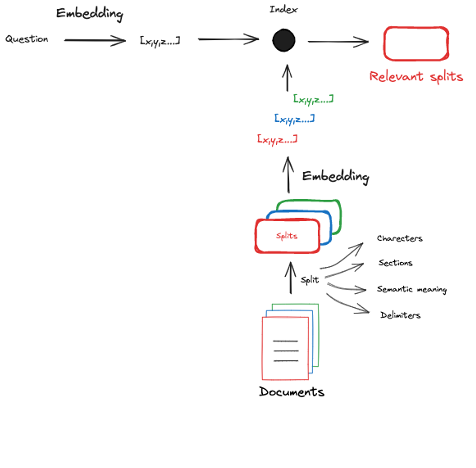
\includegraphics[width=\linewidth]{firstimage.jpg}
    \caption{}
    \label{fig:indexing-process}
\end{figure}


\subsection{Splitting}

Splitting is a foundational step in the indexing pipeline of Retrieval-Augmented Generation (RAG) systems. It addresses a critical challenge in processing long-form documents—how to preserve semantic meaning while conforming to input length constraints of downstream models. The goal is to divide documents into manageable, semantically coherent chunks that can later be embedded as vector representations for retrieval.

\begin{figure}[H]
    \centering
    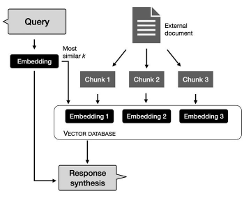
\includegraphics[width=\linewidth]{secondimage.jpg}
    \caption{}
    \label{fig:indexing-process}
\end{figure}


\subsubsection{Recursive Character-Based Splitting}

A widely adopted technique is the \texttt{RecursiveCharacterTextSplitter}, as utilized in frameworks like LangChain. This approach operates by recursively splitting text based on a prioritized list of delimiters such as paragraph breaks (\texttt{\textbackslash n\textbackslash n}), single line breaks (\texttt{\textbackslash n}), spaces (\texttt{ }), and finally, at the character level. This recursive logic ensures that the largest possible semantically coherent units are preserved while still adhering to predefined \texttt{chunk\_size} limits. 

For example, a chunk size of 1000 characters with an overlap of 200 characters is a common configuration to maintain continuity between adjacent chunks.

\begin{lstlisting}[style=mypython]
# Split Documents
text_splitter = RecursiveCharacterTextSplitter(
    chunk_size=1000, chunk_overlap=200
)

splits = text_splitter.split_documents(docs)
# Now `docs` contains chunks of text that are ready for embedding and indexing
\end{lstlisting}

This method ensures that important semantic boundaries, such as paragraph or sentence breaks, are respected as much as possible before falling back to more aggressive splitting criteria. As demonstrated in LangChain’s \textit{rag-from-scratch} repository, this process results in chunks that are better suited for embedding and semantic search tasks.


\subsubsection{Token-Aware Chunking with Overlap}

Another popular strategy is chunking by tokens, particularly with overlapping segments. Overlap is essential in preserving contextual information, especially for transformer-based models where the position of a token within its context heavily influences its representation. By ensuring that adjacent chunks share a fixed number of tokens—often referred to as a \textit{sliding window}—the model can capture cross-boundary semantics that might otherwise be lost. This method is particularly useful in scenarios where precision in retrieval is paramount, as it prevents fragmentation of key phrases or ideas that span multiple sentences.

\subsubsection{Structure-Aware Chunking}

More advanced methods adopt a \textbf{structure-aware strategy} that aligns chunks with syntactic units such as sentences or paragraphs. This is especially useful in tasks where fine-grained semantic relationships matter, such as question answering or summarization. In structure-aware models, small text units (e.g., a sentence) are treated as atomic retrieval elements, but their broader meaning is interpreted in the context of surrounding units. Thallys Costalat (2024) emphasizes that such methods yield higher retrieval precision, as the coherence of the chunk directly correlates with its informativeness during retrieval. Sentence-based chunking, for example, can be extended with ``context windows'' by appending neighboring sentences, creating composite chunks that balance granularity and context.



\subsection{Splitting Strategy Summary}

\begin{table}[H]
\centering
\begin{tabular}{|p{0.25\linewidth}|p{0.28\linewidth}|p{0.38\linewidth}|}
\hline
\textbf{Splitting Strategy} & \textbf{Key Feature} & \textbf{Use Case Scenario} \\
\hline
Recursive Character TextSplitter & Flexible-fallback through-delimiters & General-purpose chunking-of-large documents \\
\hline
TokenOverlap Chunking & Preserves continuity across segments & Semantic search with transformers-(e.g., BERT, GPT) \\
\hline
Structure-Aware Chunking & Aligns with linguistic structure & High-precision- retrieval or summarization tasks \\
\hline
\end{tabular}
\caption{}
\label{tab:splitting-strategies}
\end{table}



Each technique addresses a different trade-off between semantic preservation, context integrity, and chunk manageability. Selecting an appropriate method depends on the downstream task, document type, and retrieval sensitivity.

\subsection{Embedding}

After documents are split into semantically coherent chunks, the next stage in the RAG indexing pipeline is embedding, which transforms textual data into numerical vector representations. These embeddings allow for efficient semantic comparison, search, and retrieval within high-dimensional vector spaces.

\subsection{Purpose of Embedding}

Embedding serves as a bridge between unstructured textual information and structured numerical computation. By encoding each chunk into a dense vector, embedding models enable similarity comparisons based on vector proximity (e.g., cosine similarity or dot product), rather than relying solely on keyword overlap. This transformation is essential because it allows RAG systems to compare the semantic meaning of queries and documents, rather than just their surface-level lexical content This transformation is essential because it allows RAG systems to compare the semantic meaning of queries and documents, rather than just their surface-level lexical content.

\subsection{Types of Representations}

There are two principal methods for representing text:

\begin{itemize}
    \item \textbf{Statistical Representations:} Techniques like Bag-of-Words (BoW) and TF-IDF produce sparse vectors, which are simple but often fail to capture semantic nuance.
    \item \textbf{Machine-Learned Embeddings:} Transformer-based models like DPR (Dense Passage Retrieval), ColBERT, RAPTOR, and CONTRIEVER generate dense vectors, which embed semantic meaning into a compact numerical format suitable for neural retrieval methods.
\end{itemize}

\begin{figure}[H]
    \centering
   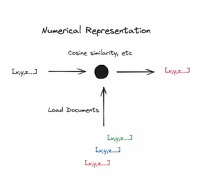
\includegraphics[width=0.85\linewidth]{thirdimage.jpg}
    \caption{}
    \label{fig:indexing-process}
\end{figure}



The latter is the standard in RAG systems due to its superior performance in understanding context, paraphrasing, and semantic similarity.

\begin{figure}[H]
    \centering
    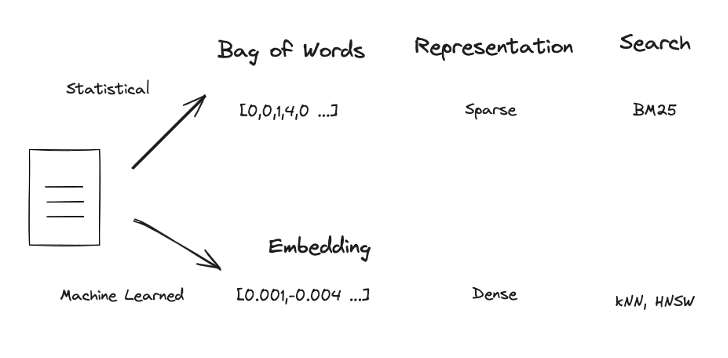
\includegraphics[width=\linewidth]{fourthimage.jpg}
    \caption{}
    \label{fig:indexing-process}
\end{figure}

\subsection{Common Embedding Models}

\begin{itemize}
    \item \textbf{DPR:} Generates a single vector per passage, optimized for full-document semantic similarity.
    \item \textbf{ColBERT:} Computes token-level embeddings, allowing fine-grained interaction between queries and passages, ideal for high-resolution retrieval.
    \item \textbf{RAPTOR:} Leverages hierarchical encoding and retrieval patterns for multi-hop reasoning.
    \item \textbf{CONTRIEVER:} Focuses on unsupervised learning of sentence-level representations, suitable for low-resource or domain-adaptive scenarios.
\end{itemize}

\subsection{Embedding Challenges}

\begin{enumerate}
    \item \textbf{High Dimensionality:} Embedding vectors typically exist in hundreds or thousands of dimensions. Searching or comparing vectors in such high-dimensional spaces is computationally intensive. Classical structures like KD-trees degrade rapidly beyond 10 dimensions.
    
    \item \textbf{Approximate vs. Exact Search:}
    \begin{itemize}
        \item \textbf{Exact Nearest Neighbor Search} guarantees precision but scales poorly.
        \item \textbf{Approximate Nearest Neighbor Search (ANNS)}—as used in libraries like FAISS—sacrifices some accuracy for speed and scalability. Tuning these systems is non-trivial and often domain-specific.
    \end{itemize}
    
    \item \textbf{Incompatible Representations:} 
    Not all embeddings are interoperable. For instance:
    \begin{itemize}
        \item \textbf{ColBERT} produces embeddings at the token level, optimized for fine-grained matching.
        \item \textbf{DPR} represents entire passages with a single embedding.
    \end{itemize}
    These differences mean that one cannot interchangeably use embeddings from different models within the same vector store. Each embedding model encodes information at a different granularity and semantic level, affecting retrieval performance and indexing compatibility.
\end{enumerate}

\subsection*{Embedding Models Comparison}

\begin{table}[H]
\centering
\begin{tabular}{|p{0.22\linewidth}|p{0.22\linewidth}|p{0.22\linewidth}|p{0.28\linewidth}|}
\hline
\textbf{Model} & \textbf{Granularity} & \textbf{Search Type} & \textbf{Use Case} \\
\hline
DPR & Passage-level & Dense vector search& General-purpose-retrieval \\
\hline
ColBERT & Token-level & Late interaction model& Fine-grained, high-precision retrieval \\
\hline
RAPTOR & Hierarchical & Hybrid & Multi-hop-or layered reasoning \\
\hline
CONTRIE-VER & Sentence-level & Dense unsupervised & Domain adaptation \\
\hline
\end{tabular}
\caption{}
\label{tab:embedding-models}
\end{table}


\section{Retrieval}
\section{Experimental Results}

\section{Conclusion}

\bibliographystyle{plain}
\bibliography{references}

\end{document}